
%(BEGIN_QUESTION)
% Copyright 2011, Tony R. Kuphaldt, released under the Creative Commons Attribution License (v 1.0)
% This means you may do almost anything with this work of mine, so long as you give me proper credit

For a moving fluid passing through any {\it heat exchanger}, the rate of heat transfer ($dQ \over dt$) required to change the temperature ($\Delta T$) of the fluid flowing at a known mass flow rate ($dm \over dt$) having a fixed specific heat value ($c$) is predicted by this formula:

$${dQ \over dt} = {dm \over dt}c \Delta T$$

\noindent
Where,

$dQ \over dt$ = Heat transfer rate (metric calories per second or British BTUs per second)

$dm \over dt$ = Mass flow rate of fluid (metric grams per second or British pounds per second)

$c$ = Specific heat of substance (typically a constant value for that substance, in BTU per pound-degree F or calories per gram-degree C)

$\Delta T$ = Temperature change (metric degrees Celsius or British degrees Fahrenheit)

\vskip 10pt

We may apply this formula to the application of a solar air heater, using the sun's radiant energy ($dQ \over dt$) to raise the temperature ($\Delta T$) of air flowing ($dm \over dt$) from the inlet to the outlet of the collector:

$$\includegraphics[width=15.5cm]{i01777x01.eps}$$

Based on this equation, determine whether the temperature rise ($\Delta T$) for any given intensity of sunlight ($dQ \over dt$) will be a self-regulating, integrating, or runaway process variable with respect to the air's mass flow rate ($dm \over dt$).  For example, if we were to suddenly increase the fan's speed to cause a greater mass flow rate of air to go through the collector, would the temperature difference settle at some new stable value (self-regulating), would it continue to change steadily over time (integrating), or would it change faster and faster over time (runaway)?

\vskip 20pt \vbox{\hrule \hbox{\strut \vrule{} {\bf Suggestions for Socratic discussion} \vrule} \hrule}

\begin{itemize}
\item{} Why would anyone care what this solar collector's characteristic response to a change in air flow would be?
\item{} This problem is one lending itself well to a {\it thought experiment}.  Describe the thought experiment you would ``perform'' on this system to explore its characteristics, and how you would apply the experiment to the equation relating heat and temperature.
\item{} For those students who have studied flow measurement technologies, identify any appropriate flowmeters for this process application.
\end{itemize}

\underbar{file i01777}
%(END_QUESTION)





%(BEGIN_ANSWER)

Temperature rise ($\Delta T$) is a {\it self-regulating} variable with respect to air flow as the independent variable.  The reason for this comes from a direct analysis of the given formula:

$${dQ \over dt} = {dm \over dt}c \Delta T$$

For any given amount of solar influx ($dQ \over dt$) and any given mass flow rate ($dm \over dt$), the $\Delta T$ is a predictable value, since $c$ is constant.  This means the process must be self-regulating, seeking a new $\Delta T$ value {\it on its own} for any new flow rate or for any new solar influx.


%(END_ANSWER)





%(BEGIN_NOTES)


%INDEX% Process: solar hot-air collector process characteristics

%(END_NOTES)


